\documentclass[11pt, a4paper]{article}
\usepackage{graphicx}
\usepackage{amsmath}
\usepackage[margin=0.6in]{geometry}
\usepackage{listings}
\usepackage{float}
\usepackage{hyperref}

\title{Applied Programming Lab: Assignment 3} % Title
\author{Harish R EE20B044} % Author name
\date{\today} % Date for the report

\begin{document}
    \maketitle % Insert the title, author and date
    \tableofcontents
    \clearpage
    

    \section{Abstract}
        The primary aim of the exercise is to study how the \textbf{amount of noise} affects the quality of estimation in the process of fitting models (linear here) to data. Further we also learn how to \textbf{extract useful information} by analyzing the data and present the same through various kinds of plots. In the  of doing so, we learn the usage of various libraries in python useful for data analysis and visualization.
    \section{Introduction}
        Our interest here is the special case of model parameter estimation, where the model is \emph{linear in parameters}, i.e,
        \begin{equation}
            f(t;p_1, p_2,..,p_N) = \sum_{i=0}^{N}p_iF_i(t)
        \end{equation}
        Say, we have M data observations and N parameters to estimate, this problem clearly reduces to the inversion of a matrix problem:
        \begin{equation}
            \left(\begin{matrix}
            F_1(t_1) & F_2(t_1) & ... & F_n(t_1)\\
            F_1(t_2) & F_2(t_2) & ... & F_n(t_2)\\
            ... & ... & ... & ...\\
            F_1(t_M) & F_2(t_M) & ... & F_n(t_M)\\
            \end{matrix}\right)
            \left(\begin{matrix}
            p_1\\
            p_2\\
            ...\\
            p_N\\
            \end{matrix}\right)
            =
            \left(\begin{matrix}
            a_1\\
            a_2\\
            ...\\
            a_M\\
            \end{matrix}\right)
            \label{eq0}
        \end{equation}

        Since our real world measurements are always noisy, Accounting for the noise, we get the following matrix equation in vector form:
        \begin{equation}
            F.\vec{p} = \vec{x_0}+\vec{n} = \vec{x}
            \label{truenoiseeqn}
        \end{equation}
        
        Since a generalized solution to this problem is extremely non-trivial, We wish to simplify things by making specific assumptions about the noise present in the data:
        \begin{enumerate}
            \item The noise added to each observation $x_i$, namely $n_i$ is \emph{independent} of the noise added to any other observation.
            \item Further the noise is uniform and normally distributed, i.e, it has zero mean and a standard deviation of $\sigma$.
        \end{enumerate}
     
        Proceeding further, we try to get the best guess for \vec{p}, by minimizing the $L_2$ norm of the error that is given by:
        \begin{equation}
            \epsilon = F.\vec{p} - \vec{x}
        \end{equation}

        The norm of the error is:
        \begin{equation}
            \|\epsilon\|^2 = \epsilon^T\epsilon = ((F.\vec{p}-\vec{x})^T(F.\vec{p}-\vec{x})) = \sum_{i}\epsilon_i^2
        \end{equation}

        On plotting the error term, we would expect the surface plot to have a minimum at some point \vec{$p_0$}. When we proceed to find it by taking the gradient and setting it to zero, We get the following result:\\
        \begin{equation}
            \begin{aligned}
                \vec{p_0} = (F^TF)^{-1}F^T\vec{x}
            \end{aligned}
        \end{equation}

        This is called the \emph{Least Squares Estimates} method.\\

    \section{Procedure}
        Let us take the following function to be the true data which we are supposed to fit linearly.
        \begin{equation}
            f(t) = 1.05J_2(t)-0.105t
        \end{equation}
        where $J_2(t)$ is the \textit{Bessel function of order 2}.

        \subsection{Adding noise to the data}
            Based on our previous assumption, We add a noise series that is normally distributed, whose probability distribution is given by
            \begin{equation}
                P(n(t)|\sigma)=\frac{1}{\sqrt{2\pi\sigma^2}}e^{-\frac{n(t)^2}{2\sigma^2}} \label{eq1}
            \end{equation}
            
            The below code snippet generates 9 columns of noisy data corresponding to 9 linearly spaced values of $\sigma$ in logspace (from $10^{-3}$ to $10^{-1}$):
            \begin{verbatim}
                def generate_data():
                    N=101                           # no of data points
                    k=9                             # no of sets of data with varying noise
    
                    # generate the data points and add noise
                    t= np.linspace(0,10,N)              # t vector
                    y=1.05*sp.jn(2,t)-0.105*t       # f(t) vector
                    Y=np.meshgrid(y,np.ones(k),indexing='ij')[0] # make k copies
                    scl=np.logspace(-1,-3,k)           # noise stdev
                    n=np.dot(np.random.randn(N,k),np.diag(scl))     # generate k vectors
                    yy=Y+n                          # add noise to signal
                    
                return t,yy

            \end{verbatim}
        \subsection{The plot function}
            We extensively use the \textbf{pyplot} module from matplotlib library for various kinds of visualization. The following code snippet is a generalized plot function, when evoked with appropriate inputs, can return the plot figures:
            \begin{verbatim}
                                
                def plot_data(fn,x,y,xl,yl,title,legends=None,stdev=None,z=None,loglog=False):
                        	
                    parameters = {'axes.labelsize': 12,
                    		  'axes.titlesize': 15,
                    		  'legend.fontsize': 10,
                    		  'mathtext.fontset':'cm'}
                    
                    plt.rcParams.update(parameters)
                    fig, ax = plt.subplots(figsize =(8,8))
                    if fn=='line':
                    	ax.plot(x,y)
                    elif fn=='err':
                    	ax.errorbar(x,y,stdev,fmt='ro')
                    elif fn=='contour':
                    	cont = contour(x,y,z,20)
                    	clabel(cont, np.linspace(0.025,0.100,4), inline=True)
                    elif fn=='dashed':
                    	ax.plot(x,y,linestyle='dashed',marker='o', markersize=5)
                    
                    if loglog:
                    	ax.set_xscale('log')
                    	ax.set_yscale('log')
                    
                    if legends:
                    	ax.legend(tuple(legends), loc='upper right')
                    
                    ax.set(xlabel=xl, ylabel=yl, title=title)
                    ax.grid()
                
                return fig
            \end{verbatim}
        
        \subsection{Visualizing the noisy data}
             Using the above described plot function, we now visualize the noisy data generated. The variation in levels of noise with respect to $\sigma_i$ is apparent in the below graph.
            \begin{figure}[H]
                \centering
                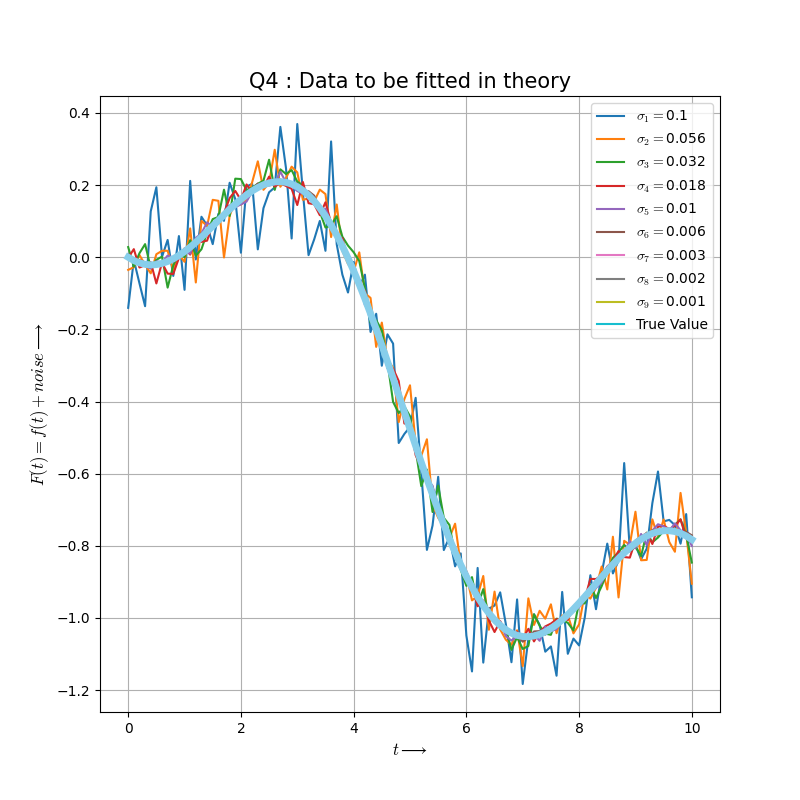
\includegraphics[scale=0.75]{noisy_data.png}
                \caption{Noisy Data with True Data}
                \label{fig:noisyAndTrue}
            \end{figure}
            
            A plot of the first column of data with error bars is also generated alongside the exact curve, by plotting every 5th data item to make the plot readable. This gives us an idea on how much the data diverges.
            \begin{figure}[H]
                \centering
                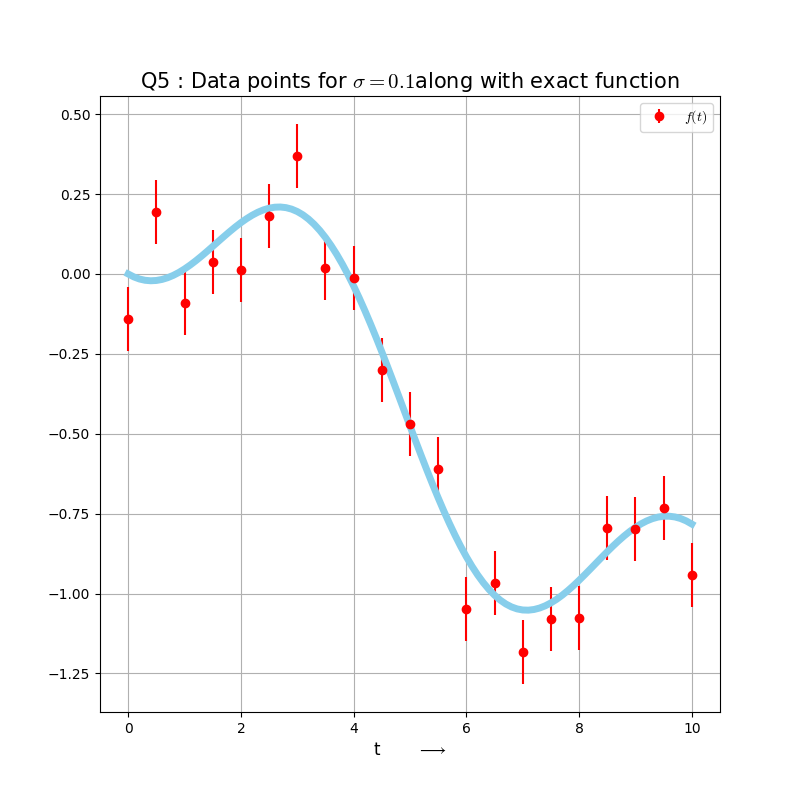
\includegraphics[scale=0.75]{error_bar.png}
                \caption{Noisy Data with Errorbar}
                \label{fig:noiseError}
            \end{figure}


        \subsection{Linear fit the data}
            The true function can be modelled as
            \begin{equation}
                g(t, A, B) = AJ_2(t)+Bt
            \end{equation}
            where $A$ and $B$ are constants that we need to find.\\

            We begin by guessing values for A and B in the ranges of $(0,2)$ and $(-2,0)$ respectively. The error in the estimate is computed as shown below            
            \begin{equation}
                \epsilon_{ij} = \frac{1}{101}\sum_{k=0}^{101}(f(t_k) - g(t_k, A_i, B_j))^2
            \end{equation}
            where $\epsilon_{ij}$ is the error for $(A_i,B_j)$.\\
            When we plot the variation of error function in the meshgrid of A and B, we find the below contour plot with a \textbf{Minima at $(A,B) = (1.1,-0.11)$} which is very close to the exact solution.
            \begin{figure}[H]
                \centering
                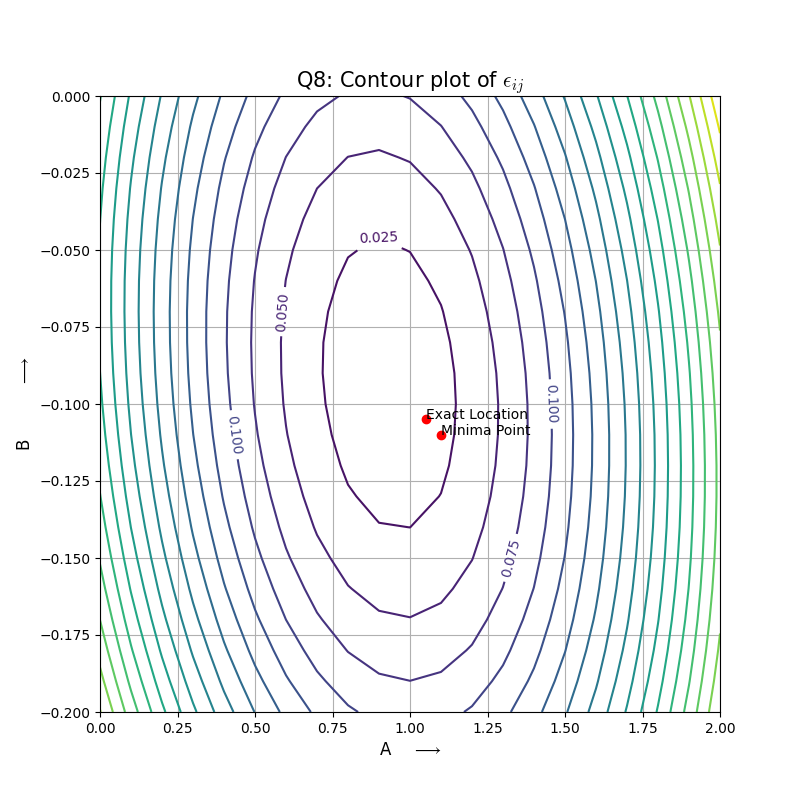
\includegraphics[scale=0.75]{contour_plot.png}  % Mention the image name within the curly braces. Image should be in the same folder as the tex file.
                \caption{Contour Plot of $\epsilon_{ij}$}
                \label{fig:contourPlot}
            \end{figure}

            As discussed earlier, we perform the least squares fit to the function using \texttt{linalg.lstsq} function available in scipy module. This solved for $A_{fit}$ and $B_{fit}$ as described by the below equation.
            \begin{equation}
            M.p = D \label{eq5}
            \end{equation}
            where
            \begin{equation}
            M=\left[\begin{matrix}
            J_2(t_1)&t_1\\
            ...&...\\
            J_2(t_m)&t_m
            \end{matrix}\right]\text{, }p=\left[\begin{matrix}
            A_{fit}\\B_{fit}
            \end{matrix}\right]\ \text{and }D=\left[\begin{matrix}f(t_1)\\...\\f(t_m)\end{matrix}\right]
            \end{equation}\\

            

        \subsection{Finding out the variation of $\epsilon$ with $\sigma_n$}
            We proceed to generate 100 different files of the \texttt{\textbf{fitting.dat}} data with different noises and get the estimates $A_{fit}$ and $B_{fit}$ using the procedure described in \emph{Section 3.3}. Then we get the mean squared error of $A_fit$ and $B_fit$ across the datafiles for a given $\sigma_i$. This MSE variation with $\sigma_n$ is captured in the below graph
            \begin{figure}[H]
                \centering
                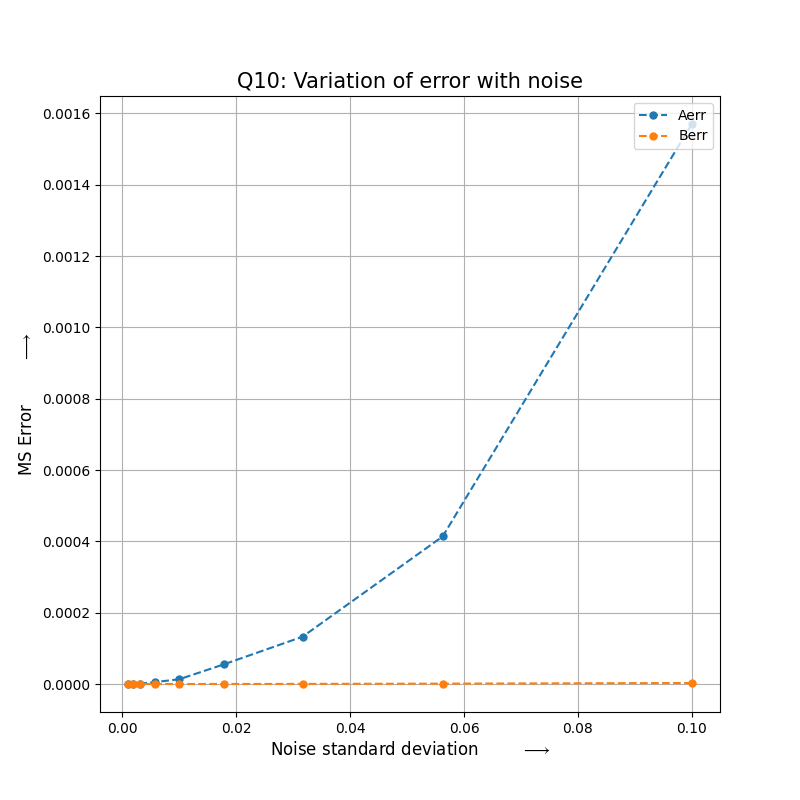
\includegraphics[scale=0.75]{error_plot.png}  % Mention the image name within the curly braces. Image should be in the same folder as the tex file.
                \caption{Mean Squared Error vs Standard Deviation}
                \label{fig:errorSTD}
            \end{figure}

            Since the above plot is not directly inferential in nature, We plot the same in \texttt{loglog} scale as below:
            \begin{figure}[H]
                \centering
                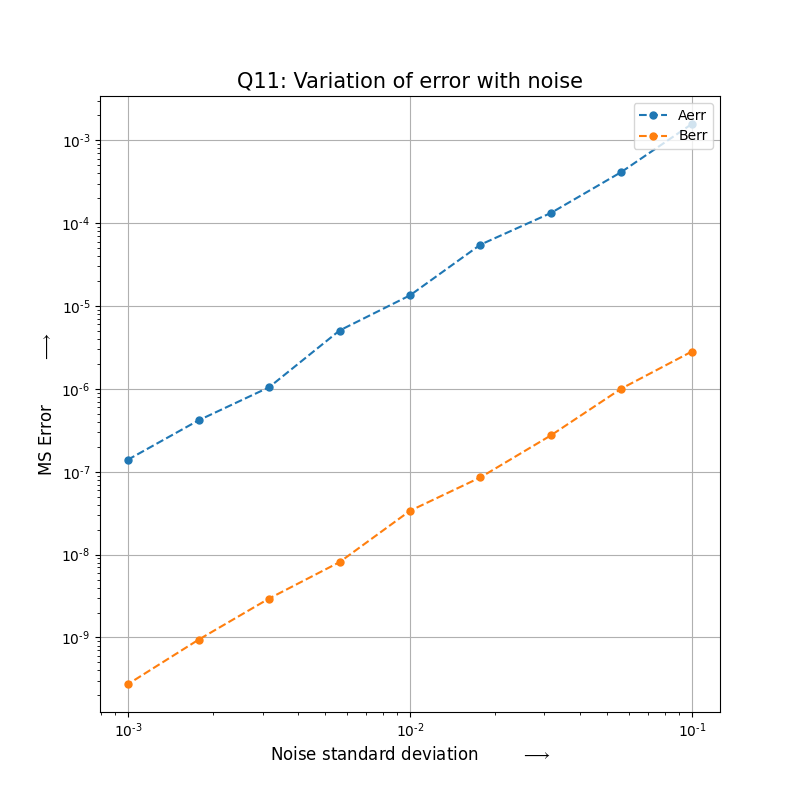
\includegraphics[scale=0.75]{error_plot_loglog.png}  % Mention the image name within the curly braces. Image should be in the same folder as the tex file.
                \caption{Error vs Standard Deviation \texttt{loglog} Plot}
                \label{fig:errorSTDloglog}
            \end{figure}

            It is evident from the above graph that the relationship between $log(\epsilon_{std})$ and $log(\sigma_{data})$ is approximately linear.

    \section{Conclusion}
        We can conclude from the exercise that, the logarithm of error in the least squares fit estimate is \textbf{linearly} proportional to the standard deviation of noise in the data.
    
    \section{Acknowledgement}
        The following sources were referred while preparing the report:
        \begin{enumerate}
            \item \textit{Section: Linear Fitting to Data}, Assignment Handout, EE2703.
            \item \textit{MathTex : \LaTeX for Matplotlib},( \href{{https://matplotlib.org/stable/tutorials/text/mathtext.html}}{MathTex Documentation})
        \end{enumerate}
\end{document}
